\markboth{Discharge curves}{Discharge curves}
\section{Discharge curves} \label{sec:dischargeCurves}
Many battery data sheets provide measured discharge curves, on which the charging and discharging behaviour of this model is based. Rather than determining the curves according to the internal impedance, a common approach \cite{lijun_gao_dynamic_2002}, this model determins the curves directly by means of digitizing the images and creating a curve fit. The classes used for fitting and modelling the discharge curves are described in the following subsections.

\subsection{Single discharge curve}
For modelling a single discharge curve, the class \mcode{dischargeFit} is used, which implements the interface \mcode{curveFitInterface}\todo{Section describing interface, etc.}. The curve is fitted according to \cite{werder_entwicklung_2014}, using a function that is loosely based on the Nernst equation with two exonential functions superimposed as a correction for the voltage drops at the beginning and end of the curve.
\begin{equation}
\begin{aligned}
V(SoC) = x_1 - \frac{R\cdot T}{z\subi{Li}\cdot F}\cdot ln\Big(\frac{SoC}{1-SoC}\Big)
+ x_2\cdot SoC + x_3 \\
+ (x_4 + (x_5 + x_4\cdot x_6)\cdot SoC)\cdot exp(-x_6\cdot SoC) \\
+ x_7\cdot exp(-x_8\cdot SoC)
\end{aligned}
\end{equation}

where $x_1,\ ..,\ x_8$ are the fit parameters, $R = 8.3144598$ J/(mol $\cdot$ K) is the universal gas constant, $z\subi{Li} = 1$ is the ionic charge number of lithium, $F = 96485.3328959$ As/mol is the Faraday constant, $SoC$ is the state of charge, $V$ is the voltage in V and $T$ is the temperature in K at which the curve was recorded. The curves are fitted using the levenberg-marquardt algorithm and either the \mcode{lsqcurvefit} method, the \mcode{fminsearch} method or a combination of both, depending on the user's preference. 

\subsubsection{Creation of a \mcode{dischargeFit} object}
A \mcode{dischargeFit} object is created with the digitized raw data - the voltage $V$ in V, the discharge capacity $C\subi{dis}$ in Ah, the current $I$ in A at which the curve was recorded and the temperature $T$ in K at which the curve was recorded.
\begin{lstlisting}
d = dischargeFit(V, C_dis, I, T);
\end{lstlisting}
\mcode{V} and \mcode{C_dis} are vectors containing the digitized raw data from the data sheet. Further options, such as initial values for the fit parameters $x_1,\ ..,\ x_8$ and the fit method can be passed to the constructor using Matlab's name-value pair syntax:
\begin{lstlisting}
d = dischargeFit(V, C_dis, I, T, 'OptionName', OptionValue);
\end{lstlisting}
By default, the initial fit parameters are set to zero and the curve is fit by first using \mcode{lsqcurvefit}, followed by \mcode{fminsearch}. The initial fit parameters are stored in a vector \mcode{x0} of \mcode{length} 8, which can be passed via the option name \mcode{'x0'}, for example using the following syntax:
\begin{lstlisting}
x0 = ones(8, 1);
d = dischargeFit(V, C_dis, I, T, 'x0', x0);
\end{lstlisting}
The method used for the curve fitting can be passed to the constructor using the option name \mcode{'mode'}. The corresponding value must be one of the following three strings:
\begin{itemize}
	\item \mcode{'lsq'} for \mcode{lsqcurvefit}
	\item \mcode{'fmin'} for \mcode{fminsearch}
	\item \mcode{'both'} for \mcode{lsqcurvefit} followed by another fit using \mcode{fminsearch}
\end{itemize}
e.g.
\begin{lstlisting}
d = dischargeFit(V, C_dis, I, T, 'mode', 'fmin');
d.plotResults
\end{lstlisting}
Depending on the curve and on the technology, one of the methods may return a better result.

\subsubsection{Visual validation}
A visual validation can be performed by calling the class's \mcode{plotResults} method (see above). In Figure~\ref{fig:dischargeFit01}, the results of two \mcode{dischargeFit} objects using the same raw data are compared.
\begin{figure}[b!]
	\captionsetup{type=figure}
	\centering
	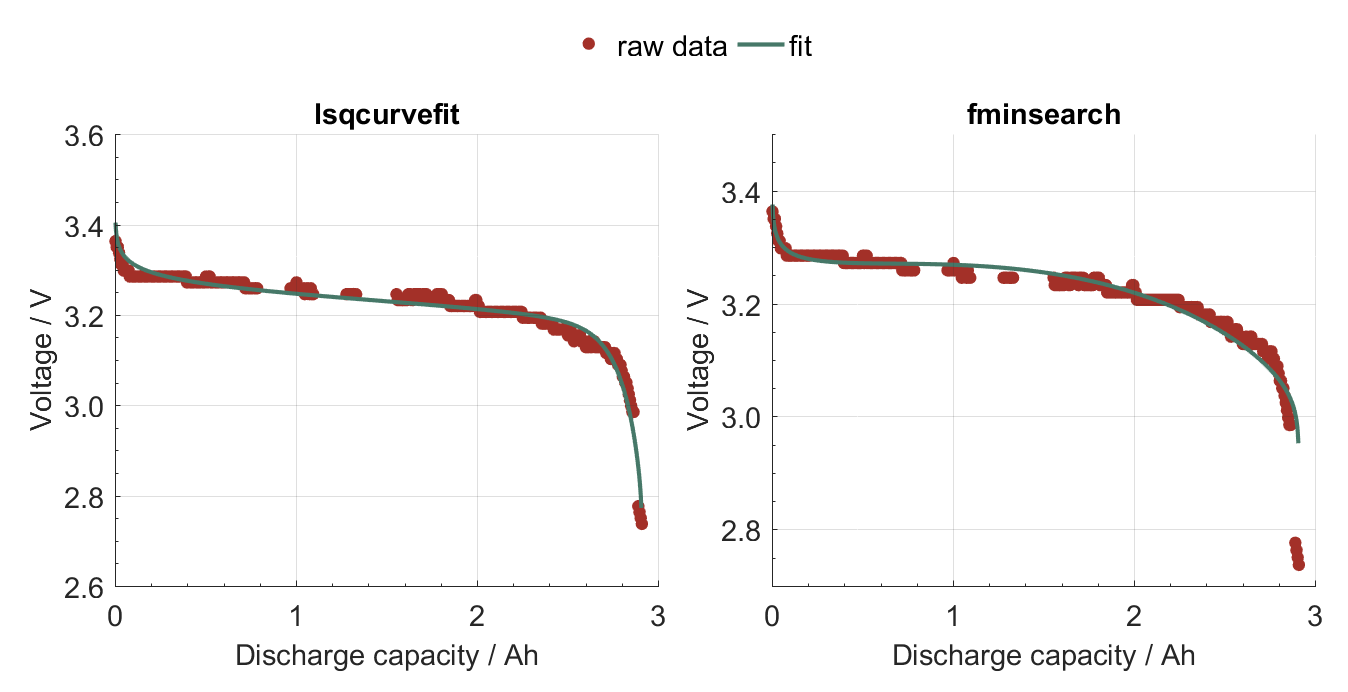
\includegraphics[width=.97\textwidth]{dischargeFit01}
	\caption[Fit results of the \mcode{dischargeFit} class using the fit methods \mcode{lsqcurvefit} and \mcode{fminsearch}, respectively]{Fit results of the \mcode{dischargeFit} class using the fit methods \mcode{lsqcurvefit} and \mcode{fminsearch}, respectively. The raw data was extracted from \cite{_data_2010}.}
	\label{fig:dischargeFit01}
\end{figure}
\begin{figure}[t!]
	\captionsetup{type=figure}
	\centering
	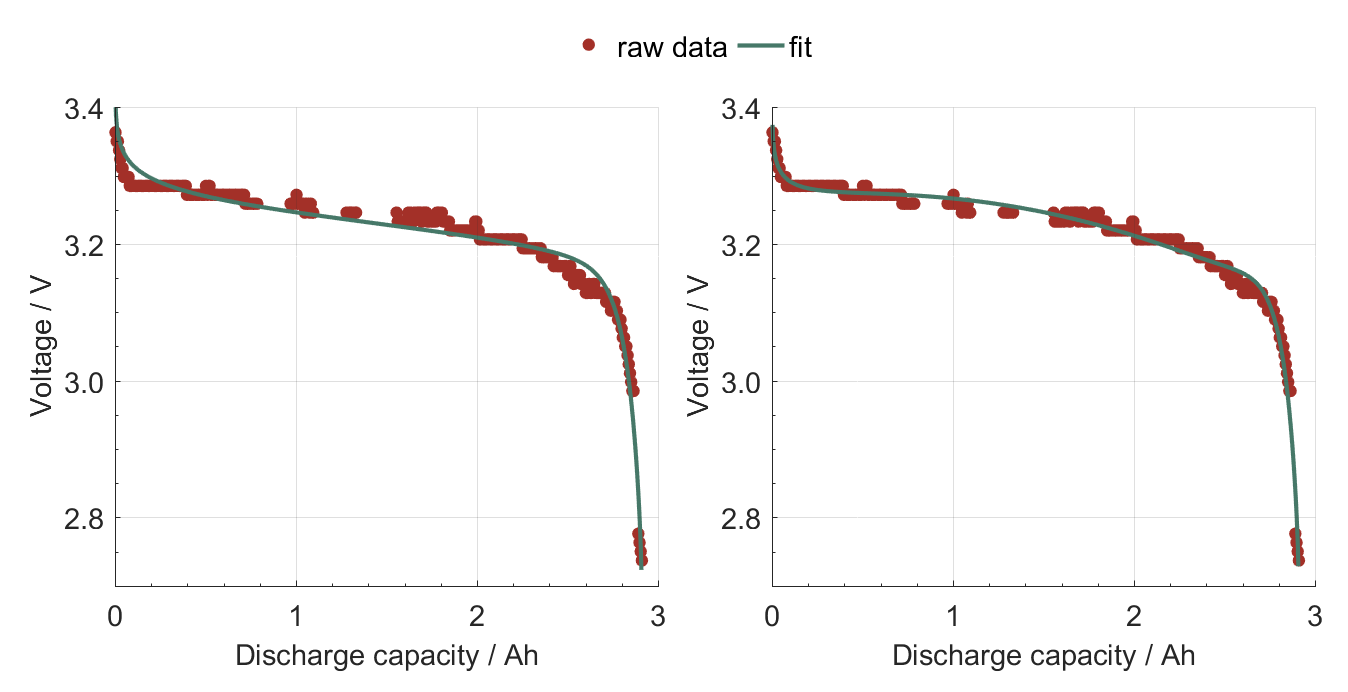
\includegraphics[width=.97\textwidth]{dischargeFit02}
	\caption[Fit results of the \mcode{dischargeFit} class using the fit mode \mcode{'both'} with the default parameter initialization and with a custom parameter initialization]{Fit results of the \mcode{dischargeFit} class using the fit mode \mcode{'both'} with the default parameter initialization (left) and with a custom parameter initialization (right). The raw data was extracted from \cite{_data_2010}.}
	\label{fig:dischargeFit02}
\end{figure}

In this example, \mcode{'lsq'} appears to return better results for the voltage drop at the end of the curve, while \mcode{'fmin'} results in a more precise fit for the voltage drop at the beginning of the curve. Further differences can be seen in the fits' curvatures. 
The \mcode{'lsq'} option results in a slightly flatter curve than the \mcode{'fmin'} mode. The results of a \mcode{dischargeFit} object using the \mcode{'both'} option are presented in Figure~\ref{fig:dischargeFit02}.
Using the default fit parameter initialization of \mcode{zeros} (left) appears to improve the curvature and voltage drops slightly, compared to the other modes. Further improvements can be made by passing custom initial fit parameters to the constructor via the option \mcode{'x0'} (see Figure~\ref{fig:dischargeFit02}, right).

\subsubsection{Object properties}
Further fit quality analysis can be performed via the mean difference in voltage between the raw data and the curve fit at the respective positions of the raw data $\overline{\Delta V}$ in V and the maximum difference between the raw data and the curve fit at the respective positions $\Delta V\subi{max}$ in V. Additionally, every curve fit class (i.e. \mcode{dischargeCurves}, \mcode{woehlerFit}, etc.) in this package implements the \mcode{curveFitInterface}, which contains the root mean square error $rmse$ as a property.
The $rmse$ for a curve fit with the raw data $y\subi{raw}$ and the fitted data $y\subi{fit}$ at the same respective $x$ coordinates is defined as
\begin{equation}
rmse = \sqrt{\frac{\sum_{i = 1}^{n}(|y\subs{raw}{i}-y\subs{fit}{i}|)^2}{n}}
\end{equation}
where $i$ is the index of the measurement and $n$ is the number of measurements. In the case of a \mcode{dischargeFit} object, $y\subs{raw}{i}$ is the measured voltage at the discharge capacity $C\subs{dis}{i}$ and $y\subs{fit}{i}$ is the fitted voltage at $C\subs{dis}{i}$. Often used for forecasting models, the $rmse$ provides a good measure of accuracy when comparing two models of the same data set~\cite{hyndman_another_2006}.
In the previous examples, the curve fit using the \mcode{'lsq'} method (Figure~\ref{fig:dischargeFit01}, left) has an $rmse$ of 0.0244~V. Using the \mcode{'fmin'} mode (Figure~\ref{fig:dischargeFit01}, right) improves the $rmse$ to a value of 0.0162~V and using the fit mode \mcode{'both'} (Figure~\ref{fig:dischargeFit02}, left) further improves it to 0.0157~V.  The lowest $rmse$ (0.0106~V) is achieved with the custom fit parameter initialization (Figure~\ref{fig:dischargeFit02}, right). \\
A list of the class's accessible properties is provided in Table~\ref{tab:dischargeFitProps}. The \mcode{z} property is inherited from the \mcode{curveFitInterface}. Setting the \mcode{x} or \mcode{mode} properties will cause the object to re-run the fitting algorithm, thus likely resulting in different values for \mcode{x} than were set by the user.

\begin{table}%[b]
	\centering
	\caption[Accessible properties of the \mcode{dischargeFit} class]{Accessible properties of the \mcode{dischargeFit} class.}
	\begin{tabular}{llll}
		\toprule
		Name & Description & Unit & Set access \\
		\midrule
		\mcode{x} & 8x1 vector of fit parameters & - & public \\
		\mcode{dV_mean} & Mean voltage difference between raw data and fit & V & read only \\
		\mcode{dV_max} & Max voltage difference between raw data and fit & V & read only \\
		\mcode{T} & Temperature at which the curve was recorded & K & immutable \\
		\mcode{z} & Current of the curve & A & immutable \\
		\mcode{mode} & Method used for fitting (\mcode{'fmin'}, \mcode{'lsq'} or \mcode{'both'})& - & public \\
		\mcode{rmse} & Root mean square error & V & read only \\
		\bottomrule
	\end{tabular}
	\label{tab:dischargeFitProps}
\end{table}

\subsubsection{Usage of a \mcode{dischargeFit} object}
In order to calculate a voltage for a given discharge capacity, the object can be treated like a function handle, by using \mcode{subsref} indexing.
\begin{lstlisting}
d = dischargeFit(V, C_dis, I, T, 'mode', 'fmin');
Cd = 1.5; % Discharge capacity in Ah
V = d(Cd); % Voltage in V
Cd_vect = linspace(0, 3, 1000); % Vector of discharge capacities in Ah
V_vect = d(Cd_vect); % Corresponding vector of voltages in V
\end{lstlisting}
A \mcode{dischargeFit} object is not accessed directly by the battery model, but rather stored in a \mcode{dischargeCurves} object. After creating a \mcode{dischargeFit}, it can be added to a \mcode{dischargeCurves} collection by using the \mcode{add()} method (see section~\ref{sec:dischargeCurves}). Alternatively, it can be added directly to a subclass of the \mcode{batteryInterface} (see section) \todo{section ref} using it's \mcode{addcurves()} method. \\

\subsection{Collection of discharge curves}
\label{sec:dischargeCurves}
A single discharge curve can be used to model the behaviour of a battery for a given current. However, in reality, a battery will often be charged or discharged with different currents. In many cases, the current may change from one simulation time step to another. In order to be able to determine the voltage as a function of $C\subi{dis}$ and $I$, multiple \mcode{dischargeFit} objects are wrapped by a \mcode{dischargeCurves} object, which is described in the following sections.

\subsubsection{Creation of a \mcode{dischargeCurves} object}
There are two ways to initialize a \mcode{dischargeCurves} object. The first option is to create an empty object and using the class's \mcode{dischargeFit()} method to add curve fits. The \mcode{dischargeFit()}  method has the same syntax as the \mcode{dischargeFit} class's constructor.
\begin{lstlisting}
dC = dischargeCurves;
I = [0.6; 1; 3; 5; 10; 20]; % Vector of currents in A
T = 293; % Temperature in K
for i = 1:6
	dC.dischargeFit(raw(i).V, raw(i).Cd, I(i), T)
end
% raw is a struct array containing the measured curve data
% from the data sheet.
\end{lstlisting}
This option has the advantage of reducing clutter in the workspace. However, changing the parameters and analysing the accuracy of the individual curve fits is more complicated.
Alternatively, the \mcode{dischargeFit} objects can be created, modified and then passed to the \mcode{dischargeCurves} constructor.
\begin{lstlisting}
d1 = dischargeFit(raw(1).V, raw(1).Cd, I(1), T);
	% Quality analysis and fit perfection here...
	% More curve dischargeFit object initializations here...
d6 = dischargeFit(raw(6).V, raw(6).Cd, I(6), T);
	% Quality analysis and fit perfection here...
dC = dischargeCurves(d1, d2, d3, d4, d5, d6);
% Equivalent:
dC = dischargeCurves;
dC.add(d1)
dC.add(d2)
% ...
dC.add(d6)
\end{lstlisting}
If a \mcode{dischargeFit} is passed to a \mcode{dischargeCurves} object that already holds a reference to a \mcode{dischargeFit} with the same current, the stored reference is replaced by the new one. Similarly, if two or more \mcode{dischargeFit} objects with the same current are passed to a \mcode{dischargeCurves} constructor, the first one is ignored.

\subsubsection{Interpolation between curves}
The calculation of the voltage for any given current and discharge capacity is done via Matlab's built-in \mcode{griddedInterpolant} class, which is called from within the \mcode{interp()} method. The syntax for a \mcode{dischargeCurves} object \mcode{dC} is as follows:
\begin{lstlisting}
V = dC.interp(I, Cd);
V = interp(dC, I, Cd); % equivalent
\end{lstlisting}
Where \mcode{V} is the voltage in V, \mcode{I} is the charging or discharging current in A and \mcode{Cd} is the discharge capacity after charging or discharging in Ah. If \mcode{I} is equal to one of the stored \mcode{dischargeFit} objects' currents, \mcode{Cd} is simply passed on to the respective object, which returns the voltage. If \mcode{I} does not match any of the stored objects and either of the input arguments is not found in the object's cache, \mcode{Cd} is passed on to each of the stored \mcode{dischargeFit} references, creating a vector of voltages for the different currents. Finally, a \mcode{griddedInterpolant} is created using the sample points, \mcode{I} is passed to it and the interpolated voltage is returned and cached. The interpolation method (the default is \mcode{'spline'}) can be changed by setting the property \mcode{interpMethod}. \\
A visual validation of the interpolation using the \mcode{'linear'} and \mcode{'spline'} methods, respectively, is depicted in Figure~\ref{fig:interpMethod}. A collection of \mcode{dischargeFit} objects for six currents was created and the fit results were plotted. Then, all fits except for the one at 10~A were added to a \mcode{dischargeCurves} object. Finally, the \mcode{interp()} method was called for a current of 10~A and a range of discharge capacities, in an attempt to replicate the \mcode{dischargeFit} results using interpolation. The linearly interpolated curve (Figure~\ref{fig:interpMethod}, left) is almost identical to the fit until the beginning of the voltage drop at the end. 
\begin{figure}[hbt!]
	\captionsetup{type=figure}
	\centering
	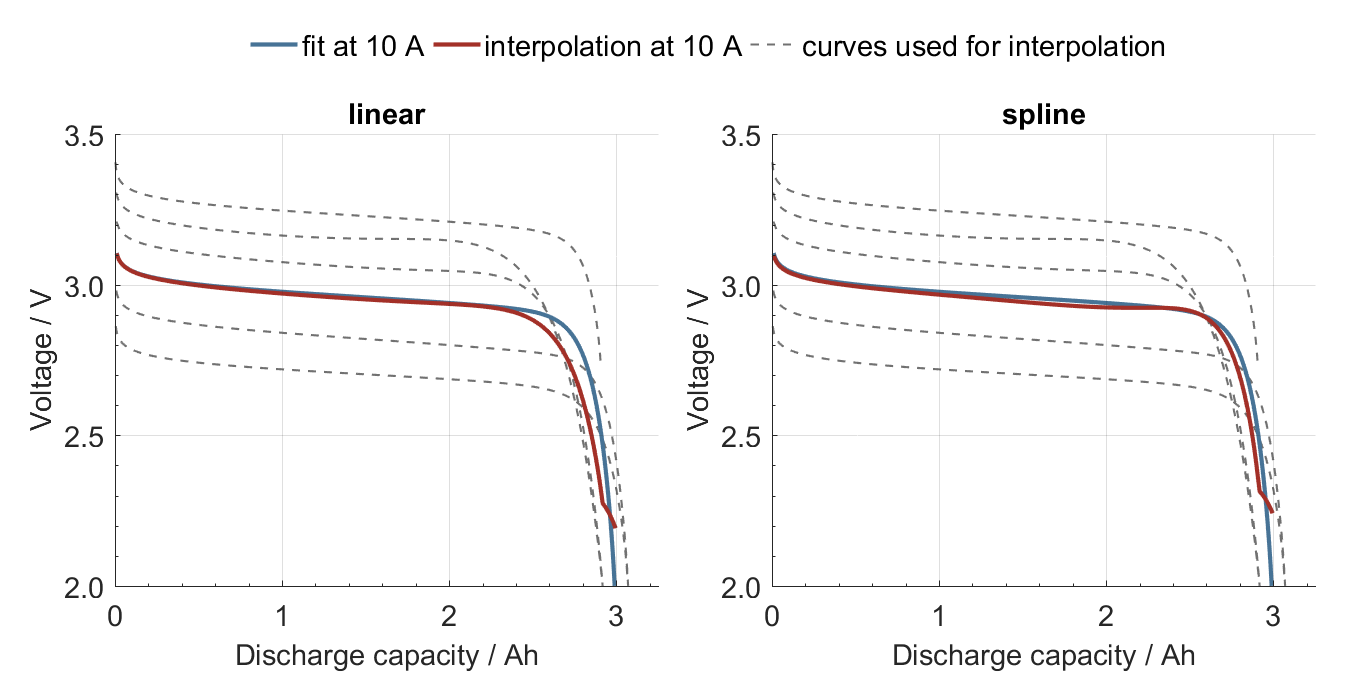
\includegraphics[width=.97\textwidth]{interpMethod}
	\caption[Comparison of the \mcode{dischargeCurves} results using linear interpolation and spline interpolation, respectively]{Comparison of the \mcode{dischargeCurves} results using linear interpolation and spline interpolation, respectively. The raw data was extracted from \cite{_data_2010}.}
	\label{fig:interpMethod}
\end{figure}
However, the spline interpolation results in an overall more precise replication of the fit if the entire curve is regarded. This indicates that the most suitable interpolation method may depend on the maximum depth of discharge $DoD$ of the modelled battery. As can be seen in Figure~\ref{fig:interpMethod}, the interpolation bends slightly at the end of the curve (close to a discharge capacity of 3~Ah). This is due to the fact that the voltage returned by a \mcode{dischargeFit} object is limited to the minimum and maximum of the raw data, respectively. If it were not limited, it could return \mcode{-Inf} or \mcode{Inf}, causing the interpolation to fail. Since most lithium ion batteries' $DoD$ are limited to 0.8 or 0.9, this bend should rarely cause any issues. \\
\begin{figure}[t!]
	\captionsetup{type=figure}
	\centering
	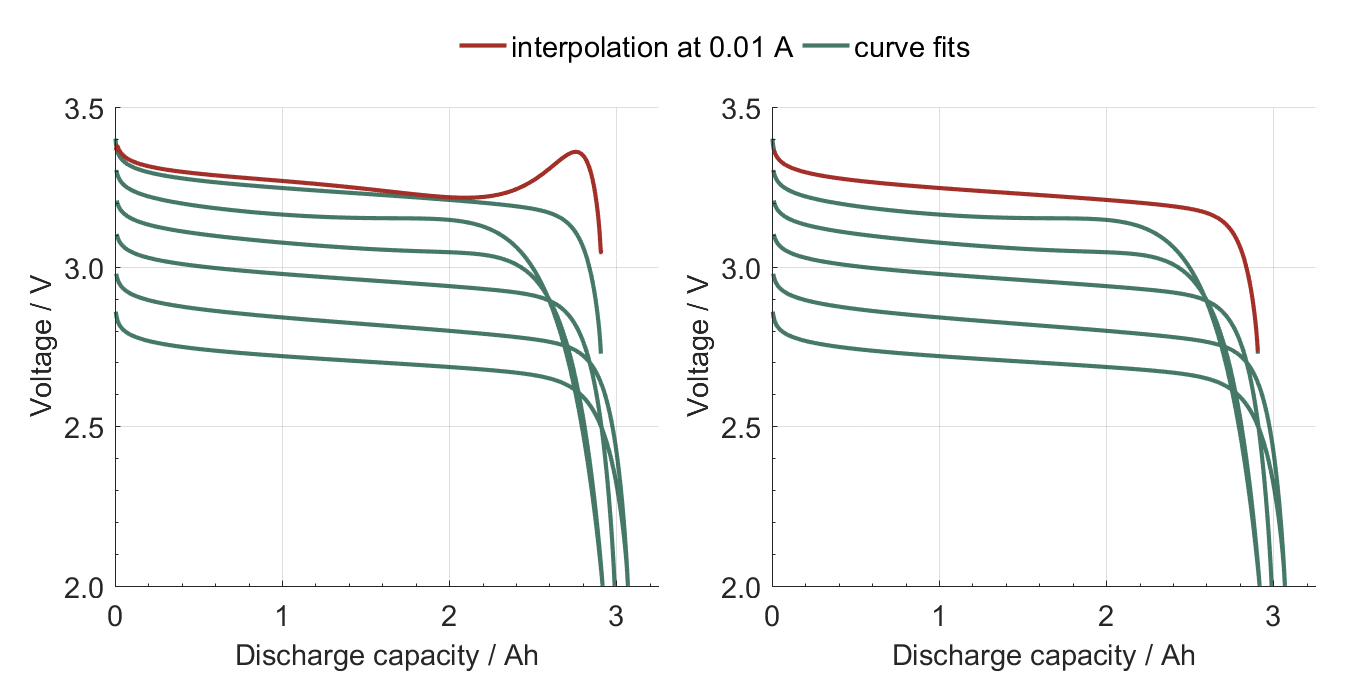
\includegraphics[width=.97\textwidth]{dischargeCurvesIlim}
	\caption[Result of the \mcode{interp()} method for a current below the lowest measured current without output limitation and with output limitation]{Result of the \mcode{interp()} method for a current below the lowest measured current without output limitation (left) and with output limitation (right). The raw data was extracted from \cite{_data_2010}.}
	\label{fig:dischargeCurvesIlim}
\end{figure}
As demonstrated Figure~\ref{fig:dischargeCurvesIlim} (left), the \mcode{interp} method using spline interpolation does not provide a good extrapolation of currents. In order to correct this, the voltage output is limited by the curve fit with the lowest current $I\subi{min}$ and by the curve fit with the highest current $I\subi{max}$, respectively. As a result, the \mcode{dischargeFit} recorded at $I\subi{min}$ is called for any current below $I\subi{min}$ (see Figure~\ref{fig:dischargeCurvesIlim}, left) and the \mcode{dischargeFit} recorded at $I\subi{max}$ is called for any current above $I\subi{max}$. In this model, the battery's maximum discharging current is limited by the \mcode{dischargeCurves} object's $I\subi{max}$ (see section\todo{ref section}).

\subsubsection{Usage of a \mcode{dischargeCurves} object}
Similarly to a \mcode{dischargeFit}, the results of a \mcode{dischargeCurves} object can be visually validated using the \mcode{plotResults()} method. Individual curve fit references removed using the \mcode{remove()} method and the respective currents. \clearpage
\begin{lstlisting}
% d = dischargeFit object
% I = current
dC.add(d) % add d to dischargeCurves dC
dC.remove(I) % remove the dischargeFit object with current I from dC
\end{lstlisting}
In order to access the \mcode{dischargeFit} references stored within a \mcode{dischargeCurves} object, the \mcode{createIterator()} method can be used. This creates an iterator object, a \matlab\ implementation of the \mcode{java.util.iterator} interface~\cite{_iterator_????}. The object can be used to iterate through the wrapped \mcode{dischargeFit} objects using a similar syntax to that of a \java\ iterator.
\begin{lstlisting}
it = dC.createIterator; % returns an scIterator object
while it.hasNext % returns true if there is another object to
				 % iterate through
	d = it.next; % returns a dischargeFit object
	% more code here
end
it.reset % resets the scIterator
\end{lstlisting}
For usage in a battery model, a \mcode{dischargeCurves} object is passed to an implementation of the \mcode{batteryInterface} (see section\todo{ref section}) using it's \mcode{addCurves()} method.